% Written by Anders Sjoqvist and Ulf Lundstrom, 2009
% The main sources are: tinyKACTL, Beta and Wikipedia

\chapter{Mathematics}

\section{Equations}

\[\begin{aligned}ax+by=e\\cx+dy=f\end{aligned}
\Rightarrow
\begin{aligned}x=\dfrac{ed-bf}{ad-bc}\\y=\dfrac{af-ec}{ad-bc}\end{aligned}\]

In general, given an equation $Ax = b$, the solution to a variable $x_i$ is given by
\[x_i = \frac{\det A_i'}{\det A} \]
where $A_i'$ is $A$ with the $i$'th column replaced by $b$.

\section{Recurrences}
If $a_n = c_1 a_{n-1} + \dots + c_k a_{n-k}$, and $r_1, \dots, r_k$ are distinct roots of $x^k + c_1 x^{k-1} + \dots + c_k$, there are $d_1, \dots, d_k$ s.t.
\[a_n = d_1r_1^n + \dots + d_kr_k^n. \]
Non-distinct roots $r$ become polynomial factors, e.g. $a_n = (d_1n + d_2)r^n$.

\section{Trigonometry}
\begin{align*}
\sin(v+w)&{}=\sin v\cos w+\cos v\sin w\\
\cos(v+w)&{}=\cos v\cos w-\sin v\sin w\\
\tan(v+w)&{}=\dfrac{\tan v+\tan w}{1-\tan v\tan w}\\
\sin v+\sin w&{}=2\sin\dfrac{v+w}{2}\cos\dfrac{v-w}{2}\\
\cos v+\cos w&{}=2\cos\dfrac{v+w}{2}\cos\dfrac{v-w}{2}
\end{align*}
\begin{align*}
	a\cos x+b\sin x&=r\cos(x-\phi)\\
	a\sin x+b\cos x&=r\sin(x+\phi)
\end{align*}
where $r=\sqrt{a^2+b^2}, \phi=\operatorname{atan2}(b,a)$.

\section{Geometry}

\subsection{Triangles}
Side lengths: $a,b,c$\\
Semiperimeter: $s=\dfrac{a+b+c}{2}$\\
Area: $A=\sqrt{s(s-a)(s-b)(s-c)}$\\
Circumradius: $R=\dfrac{abc}{4A}$\\
Inradius: $r=\dfrac{A}{p}$\\
Length of median (divides triangle into two equal-area triangles): $m_a=\tfrac{1}{2}\sqrt{2b^2+2c^2-a^2}$\\
Length of bisector (divides angles in two): $s_a=\sqrt{bc\left[1-\left(\dfrac{a}{b+c}\right)^2\right]}$\\
Law of sines: $\dfrac{\sin\alpha}{a}=\dfrac{\sin\beta}{b}=\dfrac{\sin\gamma}{c}=\dfrac{1}{2R}$\\
Law of cosines: $a^2=b^2+c^2-2bc\cos\alpha$\\
Law of tangents: $\dfrac{a+b}{a-b}=\dfrac{\tan\dfrac{\alpha+\beta}{2}}{\tan\dfrac{\alpha-\beta}{2}}$\\

\subsection{Quadrilaterals}
With side lengths $a,b,c,d$, diagonals $e, f$, diagonals angle $\theta$, area $A$ and
magic flux $F=b^2+d^2-a^2-c^2$:

\[ 4A = 2ef \cdot \sin\theta = F\tan\theta = \sqrt{4e^2f^2-F^2} \]

 For cyclic quadrilaterals the sum of opposite angles is $180^\circ$,
$ef = ac + bd$, and $A = \sqrt{(s-a)(s-b)(s-c)(s-d)}$.

\subsection{Spherical coordinates}
\centerline{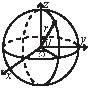
\includegraphics[width=25mm]{content/math/sphericalCoordinates}}
\[\begin{array}{cc}
x = r\sin\theta\cos\phi & r = \sqrt{x^2+y^2+z^2}\\
y = r\sin\theta\sin\phi & \theta = \textrm{acos}(z/\sqrt{x^2+y^2+z^2})\\
z = r\cos\theta & \phi = \textrm{atan2}(y,x)
\end{array}\]

\section{Derivatives/Integrals}
\begin{align*}
	\dfrac{d}{dx}\arcsin x = \dfrac{1}{\sqrt{1-x^2}} &&& \dfrac{d}{dx}\arccos x = -\dfrac{1}{\sqrt{1-x^2}} \\
	\dfrac{d}{dx}\tan x = 1+\tan^2 x &&& \dfrac{d}{dx}\arctan x = \dfrac{1}{1+x^2} \\
	\int\tan ax = -\dfrac{\ln|\cos ax|}{a} &&& \int x\sin ax = \dfrac{\sin ax-ax \cos ax}{a^2} \\
	\int e^{-x^2} = \frac{\sqrt \pi}{2} \text{erf}(x) &&& \int xe^{ax}dx = \frac{e^{ax}}{a^2}(ax-1)
\end{align*}

Integration by parts:
\[\int_a^bf(x)g(x)dx = [F(x)g(x)]_a^b-\int_a^bF(x)g'(x)dx\]

\section{Sums/Series}

\begin{comment}
\[ c^a + c^{a+1} + \dots + c^{b} = \frac{c^{b+1} - c^a}{c-1}, c \neq 1 \]
\begin{align*}
	1 + 2 + 3 + \dots + n &= \frac{n(n+1)}{2} \\
	1^2 + 2^2 + 3^2 + \dots + n^2 &= \frac{n(n+1)(2n+1)}{6} \\
	1^3 + 2^3 + 3^3 + \dots + n^3 &= \frac{n^2(n+1)^2}{4} \\
	1^4 + 2^4 + 3^4 + \dots + n^4 &= \frac{n(n+1)(2n+1)(3n^2+3n - 1)}{30} 
\end{align*}
\end{comment}
$$1^4 + 2^4 + 3^4 + \dots + n^4= \frac{n(n+1)(2n+1)(3n^2+3n - 1)}{30}$$
$$e^x = 1+x+\frac{x^2}{2!}+\frac{x^3}{3!}+\dots,\,(-\infty<x<\infty)$$
$$\ln(1+x) = x-\frac{x^2}{2}+\frac{x^3}{3}-\frac{x^4}{4}+\dots,\,(-1<x\leq1)$$
$$\sqrt{1+x} = 1+\frac{x}{2}-\frac{x^2}{8}+\frac{2x^3}{32}-\frac{5x^4}{128}+\dots,\,(-1\leq x\leq1)$$
$$\sin x = x-\frac{x^3}{3!}+\frac{x^5}{5!}-\frac{x^7}{7!}+\dots,\,(-\infty<x<\infty)$$
$$\cos x = 1-\frac{x^2}{2!}+\frac{x^4}{4!}-\frac{x^6}{6!}+\dots,\,(-\infty<x<\infty)$$

\section{Probability theory}
Let $X$ be a discrete random variable with probability $p_X(x)$ of assuming the value $x$. It will then have an expected value (mean) $\mu=\mathbb{E}(X)=\sum_xxp_X(x)$ and variance $\sigma^2=V(X)=\mathbb{E}(X^2)-(\mathbb{E}(X))^2=\sum_x(x-\mathbb{E}(X))^2p_X(x)$ where $\sigma$ is the standard deviation. 
\[\mathbb{E}(aX+bY) = a\mathbb{E}(X)+b\mathbb{E}(Y)\]
If $X,Y$ independent, \[V(aX+bY) = a^2V(X)+b^2V(Y).\]
% Expectation is linear
% If $X$ is instead continuous it will have a probability density function $f_X(x)$ and the sums above will instead be integrals with $p_X(x)$ replaced by $f_X(x)$.


\subsection{Discrete distributions}

\subsubsection{Binomial distribution}
\# of successes in $n$ independent yes/no experiments, each which yields success with probability $p$ is $\textrm{Bin}(n,p),\,n=1,2,\dots,\, 0\leq p\leq1$.
\[p(k)=\binom{n}{k}p^k(1-p)^{n-k}\]
\[\mu = np,\,\sigma^2=np(1-p)\]
$\textrm{Bin}(n,p)\approx \textrm{Po}(np)$ for small $p$.

\subsubsection{First success distribution}
The number of trials needed to get the first success in independent yes/no experiments, each wich yields success with probability $p$ is $\textrm{Fs}(p),\,0\leq p\leq1$.
\[p(k)=p(1-p)^{k-1},\,k=1,2,\dots\]
\[\mu = \frac1p,\,\sigma^2=\frac{1-p}{p^2}\]

\subsubsection{Poisson distribution}
The number of events occurring in a fixed period of time $t$ if these events occur with a known average rate $\kappa$ and independently of the time since the last event is $\textrm{Po}(\lambda),\,\lambda=t\kappa$.
\[p(k)=e^{-\lambda}\frac{\lambda^k}{k!}, k=0,1,2,\dots\]
\[\mu=\lambda,\,\sigma^2=\lambda\]

\subsection{Continuous distributions}

\subsubsection{Uniform distribution}
If the probability density function is constant between $a$ and $b$ and 0 elsewhere it is $\textrm{U}(a,b),\,a<b$.
\[f(x) = \left\{
\begin{array}{cl}
\frac{1}{b-a} & a<x<b\\
0 & \textrm{otherwise}
\end{array}\right.\]
\[\mu=\frac{a+b}{2},\,\sigma^2=\frac{(b-a)^2}{12}\]

\subsubsection{Exponential distribution}
The time between events in a Poisson process is $\textrm{Exp}(\lambda),\,\lambda>0$.
\[f(x) = \left\{
\begin{array}{cl}
\lambda e^{-\lambda x} & x\geq0\\
0 & x<0
\end{array}\right.\]
\[\mu=\frac{1}{\lambda},\,\sigma^2=\frac{1}{\lambda^2}\]

\subsubsection{Normal distribution}
Most real random values with mean $\mu$ and variance $\sigma^2$ are well described by $\mathcal{N}(\mu,\sigma^2),\,\sigma>0$.
\[ f(x) = \frac{1}{\sqrt{2\pi\sigma^2}}e^{-\frac{(x-\mu)^2}{2\sigma^2}} \]
If $X_1 \sim \mathcal{N}(\mu_1,\sigma_1^2)$ and $X_2 \sim \mathcal{N}(\mu_2,\sigma_2^2)$ then
\[ aX_1 + bX_2 + c \sim \mathcal{N}(\mu_1+\mu_2+c,a^2\sigma_1^2+b^2\sigma_2^2) \]

\section{Markov chains}
A \emph{Markov chain} is a discrete random process with the property that the next state depends only on the current state.
Let $X_1,X_2,\ldots$ be a sequence of random variables generated by the Markov process.
Then there is a transition matrix $\mathbf{P} = (p_{ij})$, with $p_{ij} = \Pr(X_n = i | X_{n-1} = j)$,
and $\mathbf{p}^{(n)} = \mathbf P^n \mathbf p^{(0)}$ is the probability distribution for $X_n$ (i.e., $p^{(n)}_i = \Pr(X_n = i)$),
where $\mathbf{p}^{(0)}$ is the initial distribution.

% \subsubsection{Stationary distribution}
$\mathbf{\pi}$ is a stationary distribution if $\mathbf{\pi} = \mathbf{\pi P}$.
If the Markov chain is \emph{irreducible} (it is possible to get to any state from any state),
then $\pi_i = \frac{1}{\mathbb{E}(T_i)}$ where $\mathbb{E}(T_i)$  is the expected time between two visits in state $i$.
$\pi_j/\pi_i$ is the expected number of visits in state $j$ between two visits in state $i$.

For a connected, undirected and non-bipartite graph, where the transition probability is uniform among all neighbors, $\pi_i$ is proportional to node $i$'s degree. \textbf{(IMPORTANT)} % https://codeforces.com/gym/101081/problem/B

% \subsubsection{Ergodicity}
A Markov chain is \emph{ergodic} if the asymptotic distribution is independent of the initial distribution.
A finite Markov chain is ergodic iff it is irreducible and \emph{aperiodic} (i.e., the gcd of cycle lengths is 1).
$\lim_{k\rightarrow\infty}\mathbf{P}^k = \mathbf{1}\pi$.

\begin{comment}
% \subsubsection{Absorption}
A Markov chain is an A-chain if the states can be partitioned into two sets $\mathbf{A}$ and $\mathbf{G}$, such that all states in $\mathbf{A}$ are absorbing ($p_{ii}=1$), and all states in $\mathbf{G}$ lead to an absorbing state in $\mathbf{A}$.
The probability for absorption in state $i\in\mathbf{A}$, when the initial state is $j$, is $a_{ij} = p_{ij}+\sum_{k\in\mathbf{G}} a_{ik}p_{kj}$.
The expected time until absorption, when the initial state is $i$, is $t_i = 1+\sum_{k\in\mathbf{G}}p_{ki}t_k$.
\end{comment}